\documentclass{beamer}

%\usepackage[utf8]{inputenc} %Para acentos en UTF8 (Prueba: � � � � � � � � � � � �)

\usepackage[latin1]{inputenc}
\usepackage[spanish]{babel}
\usepackage[absolute,overlay]{textpos}
\setlength{\TPHorizModule}{1mm}
\setlength{\TPVertModule}{1mm}

\usetheme{Warsaw}

\usecolortheme[rgb={1,0.48,0.0}]{structure}%divido los RGB por 252
\setbeamercolor{block title}{fg=white,bg=verdeuca}
\xdefinecolor{verdeuca}{rgb}{0.0,0.48,0.54}
\xdefinecolor{naranjauca}{rgb}{1,0.48,0.0}
\setbeamercolor{palette quaternary}{fg=white,bg=verdeuca}

\setbeamertemplate{navigation symbols}{}

\usepackage{color}

\title{Presentaci�n Trabajo Pr�ctico 1}
\subtitle{Arquitecturas de Aplicaciones Web}

\author[ArquiWebTeam 7]{Facundo Linari \and Franco Nicol�s Castagna}
\institute{Departamento de Computaci�n\\
Facultad de Ciencias Exactas y Naturales\\
Universidad de Buenos Aires}
\date{25-11-20}

\definecolor{celeste}{rgb}{.255,.41,.884}
\definecolor{rojo}{rgb}{1, 0, 0}

\begin{document}

\frame[plain]{\titlepage}

\begin{frame}
    \frametitle{Agenda}
    \begin{itemize}\setlength\itemsep{1em}
     \item[-] Decisiones de dise�o tomadas
     \item[-] Que componentes y m�dulos poseen, cu�les son sus responsabilidades, como se comunican entre s�
     \item[-] Presentaci�n del framework utilizado. Principales ventajas y desventajas                 
     \item[-] Que temas de dise�o y arquitectura resuelve y cu�les no. Que patrones implementa. C�mo se utiliza, que conceptos introduce.
     \item[-] Adem�s del framework utilizado, qu� otras tecnolog�as utilizaron y por qu�
     \item[-] Demo en vivo.
    \end{itemize}
\end{frame}

\begin{frame}
    \frametitle{Diagrama Entidad Relaci�n}
    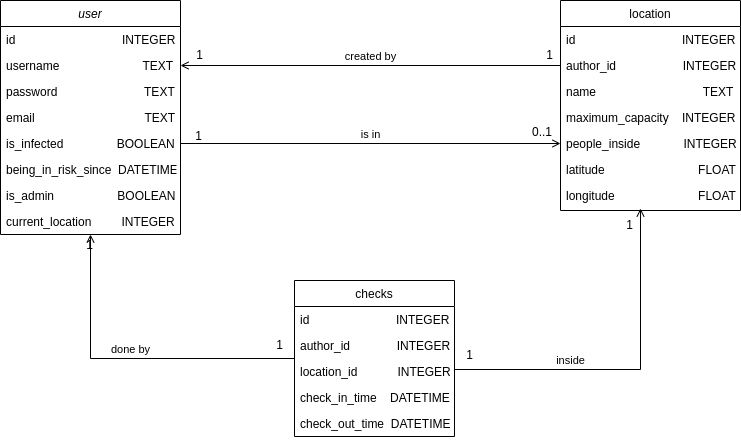
\includegraphics[width=1.0\textwidth]{img/db-entities-with-types.png}
\end{frame}

\begin{frame}
    \frametitle{Frameworks utilizados}
    Frontend:
    \begin{center}
    
\includegraphics[scale=0.3]{img/angular-logo.png}\\
    Angular
    \end{center}
    Backend:
    \begin{center}
    
\includegraphics[scale=0.3]{img/flask-logo.png}\\
    Flask
    \end{center}
\end{frame}

\begin{frame}
    \frametitle{Otras tecnolog�as}
%    \begin{itemize}
%    \item Sqlite 
\includegraphics[scale=0.05]{img/sqlite-logo.png}
%    \item Angular maps 
\includegraphics[scale=0.1]{img/angular-maps-logo.png}
%    \item Heroku 
\includegraphics[scale=0.1]{img/heroku-logo.png}
%    \end{itemize}
    \begin{tabular}{c c}
    Sqlite & 
\includegraphics[scale=0.1]{img/sqlite-logo.png} \\
    Angular maps & 
\includegraphics[scale=0.2]{img/angular-maps-logo.png} \\
    Heroku & 
\includegraphics[scale=0.2]{img/heroku-logo.png} \\
    \end{tabular}
\end{frame}

\begin{frame}
    \frametitle{JWT}
    \begin{center}
    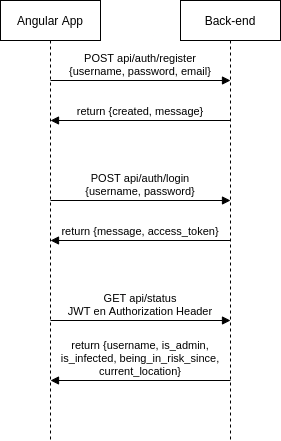
\includegraphics[scale=0.5]{img/login-with-jwt.png}
    \end{center}
    
\end{frame}

\begin{frame}
    \frametitle{Angular HttpInterceptor}
    Decorator de requests http. Incrustar token en todas las request y redirigir en caso de error. Ya sea por estar vencido el token o no tener permiso de realizar la acci�n
    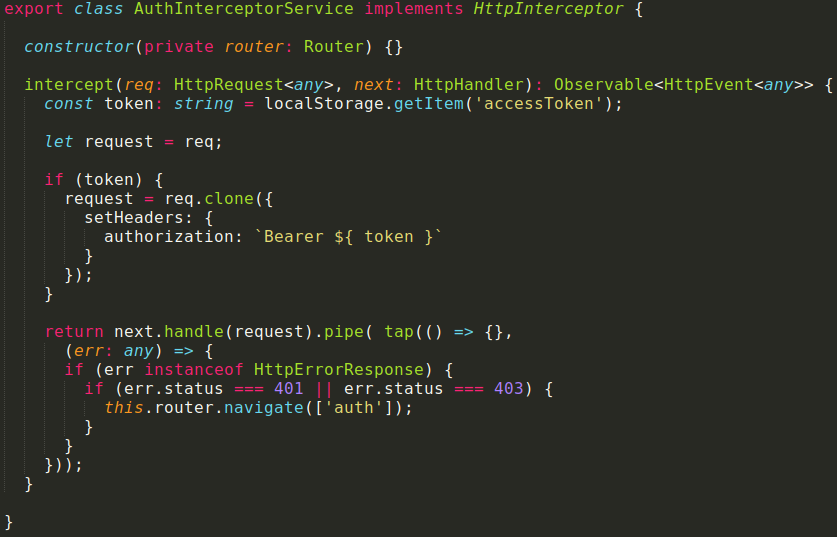
\includegraphics[width=0.9\textwidth]{img/angular-httpinterceptor.png}
    
\end{frame}

\begin{frame}
    \frametitle{Problemas tenidos}
    \begin{itemize}
    \item Al hacer el \textbf{build} de producci�n de la aplicaci�n el c�digo QR deja de funcionar
    \item No se pudo agregar \textit{Redis} porque \textit{Heroku} pide tarjeta de credito para eso
    \end{itemize}
    
\end{frame}


\begin{frame}[plain]
    \begin{center}
    \Huge ���Gracias!!! \\
    \vspace{1cm}
    \Huge �Preguntas?
    \end{center}
\end{frame}

\begin{frame}[plain]
    \begin{center}
    \Huge Demo en vivo
    \end{center}
\end{frame}

\end{document}
